%!TEX root = proposal.tex
\documentclass[11pt,letter]{article}
\usepackage[T1]{fontenc}
\usepackage{times}
\usepackage{graphicx}
\usepackage{wrapfig}
\usepackage{color}
\usepackage{xspace}
\usepackage{url}
\usepackage{subfigure}
\usepackage{algorithm2e}
\usepackage[letterpaper, top=.9in, bottom=.9in, inner=.9in, outer=.9in, foot=.25in]{geometry}
\usepackage{amsmath,amsfonts,amsthm,amssymb}
\usepackage{txfonts}
\usepackage{textcomp}
\usepackage[protrusion=true,expansion=true]{microtype}
\usepackage{array}
\usepackage{comment}
% \usepackage{multibbl}

\usepackage[compact]{titlesec}
\titlespacing{\section}{0pt}{6pt}{4pt}
\titlespacing{\subsection}{0pt}{5pt}{3pt}
\titlespacing{\subsubsection}{0pt}{5pt}{3pt}

\frenchspacing

\usepackage{listings}
\lstset{
basicstyle=\ttfamily\scriptsize,       % the size of the fonts that are used for the code
numbers=left,                   % where to put the line-numbers
numberstyle=\ttfamily,      % the size of the fonts that are used for the line-numbers
%aboveskip=0pt,
%belowskip=0pt,
stepnumber=1,                   % the step between two line-numbers. If it is 1 each line will be numbered
%numbersep=10pt,                  % how far the line-numbers are from the code
breakindent=0pt,
firstnumber=1,
%backgroundcolor=\color{white},  % choose the background color. You must add \usepackage{color}
showspaces=false,               % show spaces adding particular underscores
showstringspaces=false,         % underline spaces within strings
showtabs=false,                 % show tabs within strings adding particular underscores
frame=leftline,
tabsize=2,  		% sets default tabsize to 2 spaces
captionpos=b,   		% sets the caption-position to bottom
breaklines=false,    	% sets automatic line breaking
breakatwhitespace=true,    % sets if automatic breaks should only happen at whitespace
columns=fixed,
basewidth=0.52em,
xleftmargin=6mm,
xrightmargin=-6mm,
numberblanklines=false,
language=Ruby,
morekeywords={table,scratch,channel,interface,periodic,bloom,state,bootstrap,morph,monotone,lset,lbool,lmax,lmap},
escapeinside={(*}{*)}
}


\newcommand{\mytitle}{BIGDATA:Small:Data Collection and Management:\\Widespread CALM: Coordination Analysis and Big Data}

%%% VARIOUS COMPACTIFICATION TRICKS
% %%% CHANGE DEFAULTS
% %\setlength{\listparindent}{-170pt}}
% %\addtolength{\partopsep}{-40pt}}
% %\addtolength{\textwidth}{10mm}
% %\addtolength{\textheight}{10mm}
% \renewcommand{\baselinestretch}{0.95}
% \renewcommand{\paragraph}[1]{\vspace*{2mm}\noindent\textbf{#1} \ \ }

% ADD COMPACT OPTIONS
\newenvironment{tightitemize}{\begin{list}{$\bullet$}{\setlength{\itemsep}{1pt}\setlength{\topsep}{2pt}\setlength{\parskip}{1pt}\setlength{\parsep}{1pt}\leftmargin=1.5em}}{\end{list}}
\newcommand{\denselist}{\addtolength{\itemsep}{-7pt}}
% indent full paragraph for compact lists
\newenvironment{myparindent} {
  \hangindent=1em
  \hangafter=0
  \noindent
}

%captionsmall -- format captions in a smaller font
\newcommand{\captionsmall}[1]{\caption{\footnotesize{#1}}}
\newcommand{\myurl}[1]{{\footnotesize \url{#1}}}

% THEOREMS -------------------------------------------------------
\newtheorem{thm}{Theorem}[section]
\newtheorem{cor}{Corollary}
\newtheorem{lem}{Lemma}
\newtheorem{prop}{Proposition}
%\theoremstyle{definition}
\newtheorem{defn}{Definition}
\newtheorem{property}{Property}
%\theoremstyle{remark}
\newtheorem{rem}{Remark}
%\theoremstyle{assumption}
\newtheorem{assumpt}{Assumption}
%\numberwithin{equation}{section}
\newtheorem{example}{Example}
\newtheorem{ex}[thm]{Example}
\newtheorem{exa}{Example}
\newtheorem{dfn}{Definition}[section]
\newtheorem{goal}{Goal}

% OTHER MACROS -----------------------------
% inline comments
% color names at http://en.wikibooks.org/wiki/LaTeX/Colors#Predefined_colors
\usepackage[usenames,dvipsnames]{xcolor}
% \newcommand{\jmh}[1]{{\textcolor{red}{#1 -- jmh}}}
\newcommand{\jmh}[1]{}

% Comment out to take away comments
\newcommand{\commentout}[1]{}
\newcommand{\out}[1]{}

\newcolumntype{C}[1]{>{\centering\arraybackslash}p{#1}}

% no page numbers
\pagestyle{empty}


\def\blooml{Bloom$^L$\xspace}



\begin{document}
  
  \vspace{-2pt}
\section*{\mytitle\\
{\normalsize PI: Joseph M. Hellerstein, U.C. Berkeley}}
% 1 page
Most architects of modern Big Data infrastructure believe that perfect distributed consistency is too expensive to guarantee in the large~\cite{ladisreport}.  This issue is often discussed in the context of data storage and retrieval, but it is also a major consideration in distributed Big Data computational infrastructure as well---be it application-level business rules~\cite{finkelstein2011} or machine learning algorithms~\cite{hogwild}.  Instead, loosely consistent approaches are often considered to be a better choice, since temporary inconsistencies across machines can often be made to work out at application level.By this reasoning, coordination mechanisms (transactions, locks, quorums, barriers, etc.) should be reserved for infrequent, mission-critical tasks.  The cost of this design pattern comes in software complexity: with loosely consistent infrastructure, application programmers must reason explicitly about distributed consistency issues for each high-level application feature.

Like many well-intentioned design maxims, this one is not so easy to translate into practice; all kinds of unavoidable tactical questions pop up.  Exactly where in a multi-component system is eventual consistency “good enough”, and when is coordination truly necessary?  How can a developer know that their “mission-critical” software is not tainted by others' ``best-effort'' components?  How does an architect maintain proper design maxims as software evolves? For example, how can the junior programmer in year $n$ of a project reason about whether their piece of the code maintains the system’s overall consistency requirements?

We made some foundational breakthroughs into these thorny questions in recent years.  The \emph{CALM Theorem} proves that Consistency can be guaranteed without coordination for programs that are Logically Monotonic. CALM analysis also leads to judicious use of coordination logic: coordination serves exclusively as a guard for non-monotonic reasoning.  Following from these ideas, we developed the \emph{Bloom} programming language.  Bloom is a ``disorderly'', data-centric language that discourages programmers from dictating the order of data and operations, since such orderings are expensive to guarantee in distributed systems.  Bloom's roots in logic programming enable simple compiler checks for monotonicity, which can be used to inform programmers about when and why to use expensive coordination logic to control order.

The goal of this proposal is to \textbf{bring CALM theory to bear on the practices of Big Data developers in the Cloud}, making it easy for distributed programmers to relax their use of coordination and embrace distributed disorder in a natural yet principled fashion.  This goal requires significant research to extend the instantiation of CALM theory into the practice of building distributed systems.  


\vspace{6pt}
\noindent \textbf{Intellectual Merit.} Initial versions of CALM and Bloom have been steeped in a ``closed world'' of logic programming and low-level, fine-grained communication.  The work here proposes to extend this research to address challenges in a number of directions: \emph{modeling massive distributed storage as a software component}, including a wide variety of possible consistency semantics; \emph{analyzing monotonicity in familiar data types} that go beyond simple logic predicates and relations; \emph{composing encapsulated, service-oriented APIs using Bloom as a principled orchestration language} that can reason about the composition of API contracts; and \emph{providing CALM-aware software engineering tools} to back up these ideas with efficient debugging and testing frameworks that can help achieve and maintain software correctness over time.
 
\vspace{6pt}
\noindent \textbf{Broader Impacts.} Beyond the scientific and engineering impact of the Bloom languages and CALM analysis, this work is intended to affect the way that Big Data software is implemented in the field.  To promote understanding of these concepts and adoption of techniques, we will run a Massive Open Online Course (MOOC), to reach out not only to Berkeley students and fellow researchers, but also to developers around the world. We will also continue to engage aggressively in industry, as we have been doing in recent years.  Given our history of releasing useful software, we plan to focus a significant fraction of this effort on releasing new versions of Bloom and its compiler analyses that can be used in academia and industry, along with the course materials and videos.

% where the main components include novel
% contributions in multiple areas:
% \begin{tightitemize}
% \itembf{Visualization \& Interaction}: tools for end-user
% analysts to construct workflows, assess the results of learning
% algorithms, refine models, explore recommended alternatives, and
% provide feedback and labels.   
% \itembf{Feedback Models to Machine Learning (ML) Algorithms}: algorithms that enable analysts to go beyond
% simply labeling data, to provide new, more intuitive forms of
% \emph{constraint-based feedback};  new active learning methods
% that allow the system to make the most out of a user's attention.  
% \itembf{Hierarchical Big Data Representations}: 
% human-understandable, multi-scale abstractions of data, which
% integrate a user's interactive view
% %of the learning procedure on their desktop computer
% with anytime processing of the entire dataset in the Cloud.
% \itembf{Online Distributed Machine Learning}: algorithms that translate hierarchical representations and user feedback into anytime processing and
% solution methods with theoretical guarantees.
% \itembf{Systems Synthesis from Domain-Specific Languages
%   (DSLs)}:  integrate these layers of data processing and understanding  via task-appropriate DSLs, compiled to run efficiently in scalable distributed systems.
% \end{tightitemize}

%\joe{We may want to integrate the next two paragraphs.}
%We propose to tackle this problem with two key technical themes that cut across disciplines: (a) the design of high-level, data-centric \emph{Domain-Specific Languages} (DSLs) for data analysis tasks, and (b) \emph{mixed-initiative visual analysis interfaces} that enable analysts to specify, assess and manipulate an analysis workflow. The use of DSLs allows us to model analytic operators at a level of abstraction that is appropriate to the task, and generate lower-level code for a variety of runtime platforms. In turn, the visual interface will translate user interactions into DSL statements and orchestrate low-latency client-side processing of data samples with slower, large-scale processing in the cloud. The interface will also provide coordinated visualizations for both data and models throughout the analysis workflow.

%The design and use of DSLs form the technical cornerstone of our approach.  By isolating simple, task-appropriate DSLs, we can extract user intent at a high level in a visual or simple programmatic interface, and use a \emph{single small DSL program} to generate two semantically identical code artifacts: one appropriate for the client, the other for a distributed cloud infrastructure.  The client code works at modest scale (gigabytes) on an extract of the data and runs with interactive speed to generate a fluid user experience, while the cloud-based code works on the full data set and produces ``online'' or ``anytime'' results that can respond in finer detail to user behavior, albeit at a coarser timescale.  
% These two simultaneous runs of the program are connected bidirectionally: the cloud code (with richer data access) can provide detail to the client, and the client code (with richer human access) can provide context and information to the cloud computation.  This approach marries ideas from online query processing and anytime algorithms (backend interactivity), active learning (backend driving frontend) weakly-supervised learning (frontend driving backend) and \emph{XXX interactive HCI goodness as in Wrangler and interactive vis tools} (frontend interactivity).

%This architectural pattern is a generic approach to interacting with Big Data, and results from initial designs we have been doing for manipulating unstructured but inherently tabular data \cite{kandel:2011:wrangler}. To ground and scope the work in this proposal, we propose to focus specifically on applications in \textbf{Text Analytics}. Unlike tabular data, which can often be visualized and analyzed directly, text emphasizes the need for feature extraction and modeling in order to to generate structure suitable for analysis. We intend to focus on the concrete problems of \emph{topic modeling} (understanding latent themes in a corpus), \emph{document similarity and clustering} (categorizing or finding similar documents), and \emph{recommendation} (suggesting unread documents of interest). \textbf{Say more about how these applications relate to our technical themes?}

%\joe{Carlos' stuff is currently missing from here.  One natural thing to do is to argue that many of the ML algorithms that are relevant to text analysis we well captured in a computational abstraction centered on graphs.  This may actually help highlight the diversity of modeling challenges at both the DSL and HCI levels: the end-user goal relates to collections of text docs, but the internal representation goes through models that are described over graphs. We need to map from a text-centric DSL to a tabular or matrix DSL over features to a graph DSL to support a clean separation of concerns at the system design level.  Similarly we also need to help users map semi-intuitively from one visual metaphor to another (as Jeff describes in his section draft) at the interface level.}

%\joe{This also suggests a way to organize some sections of the proposal by ``representational domain'': start with a focus on processing collections of linear text (tokenization, CRFs, etc.), switch to a focus on extracted text features (TFxIDF and LDA input/output, etc.), and then to a focus on graphical representations (algorithm implementations in GraphLab, document clusters and proximity, user communities and content recommendation...).  In each section we can highlight a canonical use case or two, describe the representation from a DSL perspective (its structure and operations), and talk about visual representations and interaction.  Of course after doing all that we have to talk about cross-representation issues: compilation as well as the kinds of vis/interaction issues that Jeff mentions e.g. trellis of plots across representations.}  
  
\section{Introduction}
\jmh{On a later pass, make sure that thematically we push on going ``widespread''---that is, make sure we don't seem like our impact is limited to Bloom, but rather that (a) our ideas are cracking open big, general challenges, and (b) the work we're proposing applies to widely-deployed systems.}
\label{sec:intro}
\section{Introduction}
%Our research is motivated by two hard problems in distributed systems.  First,
\wrm{show examples of the problems (not necessarily code) -- evolving state and unreliable communication}

%Distributing any system introduces nondeterminism.  For example, one may
%distribute a computation over many inexpensive, but unreliable, commodity
%machines (e.g. RAID).  The status of internet links and widely distributed
%nodes is inherently more unreliable than multiple cores on a single die, or
%multiple CPUs in a single computer.  

%We present {\bf \lang}, a foundation language for programming and
%reasoning about distributed systems.  

%We correct deficiencies in earlier attempts, and introduce a compelling notion
%of non-determinism in the language.  We specifically use non-determinism to
%reason about {\em when} a deduction becomes visible, including the possibility
%that the deduction will never be visible.  Programmers can constrain this
%non-determinism by using well-studied techniques in distributed systems, such as
%Lamport Clocks 


Traditional database systems are based on declarative query languages that
specify transformations as dataflows over an updatable store.  Such query
languages are either not expressive enough to capture common programming
constructs \wrm{like what?}, or are at best awkward to use in this fashion.
\wrm{todo: transition that explains Datalog's birth from these languages... I
don't know enough to write it} The family of logic-based database languages, of
which Datalog is the progenitor, represent expressive programming languages
that produce similar dataflow representations.  Datalog is purely deductive: a
program specifies the rules by which the derived relations are populated based
on a static database, which is never updated.  Recent programming language
research has explored the use of Datalog-based languages for expressing
distributed systems.  Because the state of any complex system evolves with its
execution, these efforts were forced to extend the Datalog model by admitting
updates, additions and deletions of the EDB.  Unfortunately, these previous
attempts were plagued with ambiguities about how and when state changes occur
and become visible, putting a heavy burden on the programmer to ensure even
simple properties, such as atomicity of updates over time.

In contrast to reasoning about state change procdurally, \lang observes
that this concept is intuitively expressed as invariants over {\em time}.  In
this work, we present a formal model of Datalog augmented with time extensions.
By reifying time as data an introducing it into the logic, \lang eliminates
previous ambiguities, ensures atomicity of updates and makes it possible to
express system invariants that can guarantee liveness properties, a key
challenge in building distributed systems.


\section{Background: Bloom}
\label{sec:bg}
\section{Background}
\label{sec:jol}
\label{sec:bg}

The Overlog language is sketched in a variety of papers.  Originally
presented as an event-driven language~\cite{p2}, it has evolved a semantics more carefully grounded in Datalog, the standard deductive
query language from database theory~\cite{ullmanbook}.  Our Overlog is
based on the description by Condie et al.~\cite{evitaraced}.  We briefly 
review Datalog here, and the extensions presented by Overlog.
%%We
%%review Datalog in Appendix~\ref{app:datalog}, and the extensions
%%offered by Overlog here.

The Datalog language is defined over relational tables; it is a purely logical query language that makes no changes to the stored tables. A Datalog \emph{program} is a set of \emph{rules} or named queries, in the spirit of SQL's \emph{views}.  A Datalog rule has the form:
\[
	r_{\mbox{\em head}}(\langle\mbox{\em col-list}\rangle) \mbox{{ \tt :- }} r_1(\langle\mbox{{\em col-list}}\rangle), \ldots, r_n(\langle\mbox{{\em col-list}}\rangle)
\]
Each term $r_i$ represents a relation, either \emph{stored} (a database table)
or \emph{derived} (the result of other rules).  Relations' columns are listed as
a comma-separated list of variable names; by convention, variables begin with
capital letters.  Terms to the right of the \texttt{:-} symbol form the rule
\emph{body} (corresponding to the {\tt \small FROM} and {\tt \small WHERE}
clauses in SQL), the relation to the left is called the \emph{head}
(corresponding to the {\tt \small SELECT} clause in SQL).  Each rule is a
logical assertion that the head relation contains those tuples that can be
generated from the body relations.  Tables in the body are joined together based
on the positions of the repeated variables in the column lists of the body
terms.  For example, a canonical Datalog program for recursively computing all
paths from links~\cite{loo-sigmod06} is shown in Figure~\ref{fig:datalogsql}
(ignoring the Overlog-specific {\tt @} notation), along with an SQL translation.
Note how the SQL {\tt \small WHERE} clause corresponds to the repeated use of
the variable {\tt \small To} in the Datalog.

%\rcs{START} Overlog extends Datalog with distribution and a semantics for table updates.
%\rcs{END Between START, END isn't really true in \JOL, and is (I
%think) a confusing way to think about location specifiers.  For one
%thing, \JOL doesn't partition the tables, because it doesn't
%understand membership.  Also, \JOL supports local tables, and
%networks that contain multiple programs.  Recommend next paragraph
%instead.}
\begin{figure}[t]
%\begin{minipage}{0.5\linewidth}
\begin{footnotesize}
\begin{verbatim}
path(@From, To, To, Cost) 
        :- link(@From, To, Cost);
path(@From, End, To, Cost1 + Cost2)
        :- link(@From, To, Cost1),
           path(@To, End, NextHop, Cost2);
\end{verbatim}
\end{footnotesize}
%\end{minipage}
%\begin{minipage}{0.5\linewidth}
\begin{footnotesize}
\begin{verbatim}
WITH RECURSIVE path(Start, End, NextHop, Cost) AS
(   SELECT From, To, To, Cost FROM link
    UNION
    SELECT link.From, path.End, link.To,
           link.Cost + path.Cost
      FROM link, path
     WHERE link.To = path.Start );
\end{verbatim}
\end{footnotesize}
%\end{minipage}
\vspace{-8pt}
\caption{Example Overlog for computing all paths from links, along with an SQL translation.}
\label{fig:datalogsql}
\end{figure}


Overlog extends Datalog in three main ways: it adds notation to
specify the location of data, provides some SQL-style extensions such
as primary keys and aggregation, and defines a model for processing
and generating changes to tables.  Overlog supports relational tables
that may optionally be ``horizontally'' partitioned row-wise across a
set of machines based on a column called the \emph{location specifier},
which is denoted by the symbol {\tt @}.
%A tuple is stored at the address specified in its location specifier column.
%  \JOL generalizes this slightly by supporting ``local'' tables that have no location specifier.  This is a notational shorthand to prevent bugs: the same effect can be achieved by adding an additional location specifier column such tables, and ensuring that the value for each tuple is always ``localhost''.
%\rcs{Killed footnote; still object to saying tables are ``horizontally partitioned''.  It would be crisper/more accurate to say this:  Overlog rules contain {\em location specifiers} which are denoted by the symbol {\tt @}.  Each tuple is stored at the address specified in its location specifier column.  OPTIONALLY:  A join against a location specifier column produces a list of machines that should be involved in a rule's evaluation; a more complete discussion of rule localization is available in \cite{sigmod06xxx}}.  A subset of columns may be marked as the table's primary key, in which case no two rows may match on those columns.  By default, the primary key consists of all columns, implying that no two rows of a table may be identical.
% 
% A \JOL  network may be partitioned into sub-networks with ``private'' versions of the same table and library, or even contain different schemas and programs.  This allows us to compose \JOL services and simplifies Overlog programs that must reason about network partitioning, nodes with inconsistent data, and explicit state transfer.  
% 
%\rcs{move next sentence before primary key discussion?}
%%(Appendix~\ref{app:datalog} shows a standard network routing example from previous papers on declarative
%%networking.)
%\rcs{ cut rest of paragraph?}A location specifier column contain legal network addresses. 
% \rcs{<- This sentence isn't true: loc specifiers are ``String'' typed: if the schema knew about location specifiers, some programs would be harder to express.}  
%\JOL supports an extensible set of network address types, but we focus on IP address:port pairs in this paper.
 % corresponding to different protocols, though for this paper we implemented TCP and UDP, and hence location specifiers are on IP address:port pairs.  

%\jmh{Add a little on partitioning inducing communication, and cite SIGMOD '06 for localization.  Point out that the SQL is single-site, but the Overlog is part of a functioning routing protocol implementation.} \rcs{Does my redefinition of location specifier handle this?}

\begin{figure}[t]
  \centering
    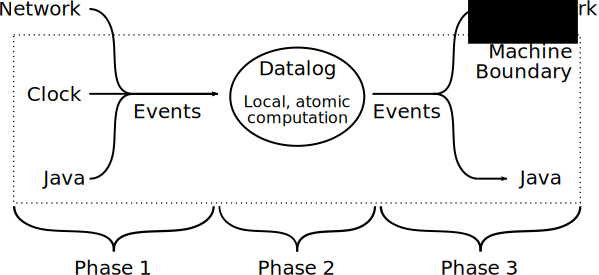
\includegraphics[width=0.95\linewidth]{jol-node.pdf}
    \label{fig:jol-node}
    \caption{An Overlog timestep at a participating node: incoming
      events are applied to local state, the local Datalog program 
      is run to fixpoint, and outgoing events are emitted.}
\vspace{-8pt}
\end{figure}

When Overlog tuples arrive at a node either through rule evaluation or
external events, they are handled in an atomic local Datalog
``timestep.'' Within a timestep, each node sees only locally-stored
tuples.  Communication between Datalog and the rest of the system
(Java code, networks, and clocks) is modeled using \emph{events}
corresponding to insertions or deletions of tuples in Datalog tables.

Each timestep consists of three phases, as shown in Figure~\ref{fig:jol-node}.
In the first phase, inbound events are converted into tuple insertions and
deletions on the local table partitions.  The second phase interprets the local rules and tuples according to traditional Datalog semantics, executing the rules to a ``fixpoint'' in a traditional bottom-up fashion~\cite{ullmanbook},
recursively evaluating the rules until no new results are generated.  In the
third phase, updates to local state are atomically made durable, and outbound
events (network messages, Java callback invocations) are emitted. Note that
while Datalog is defined over a static database, the first and third phases allow
Overlog programs to mutate state over time.

% Communication in Overlog happens as a side-effect of data partitioning. Loo et al.\ show that any Overlog program can be compiled into 
% a form where the body relations join on the same location-specifier variable, so that all relational processing is localized~\cite{loo-sigmod06}.  They also prove eventual consistency of the distributed tables under the rules, when certain simplifying assumptions hold.  In Section~\ref{sec:lessons} we discuss our experience with this model.

%\rcs{Rewrote this; the old discussion doesn't match the current implementation; the difference between the two is important for atomicity + transactions.  OLD: Each timestep consists of five phases.
% , which taken together atomically modify a local database, execute a Datalog program on that database, materialize the consequences of the program, and generate messages.  
%In Phase 1 ({\em Insertion}), inbound tuples are dequeued from a {\em network insertion queue}; each tuple arrives annotated with the name of a table, into which it is inserted\footnote{Tuples that do not conform to the local database schema are inserted into an ``exception'' table that can be configured either to store or drop tuples. \jmh{Is this a lie?}}.  In Phase 2 ({\em Datalog}), the Overlog rules in the system are treated as purely declarative Datalog queries, which are run recursively to their conclusion: a fixpoint where further application of the rules produces no new results. \JOL uses a delta-computation approach to speed up this process~\cite{matview-maintain}. In Phase 3 ({\em Materialization}), the outputs of Phase 2 queries that have the local address in their location specifier are cached in the local database as {\em Materialized Views}~\cite{matview-maintain}; output tuples with remote location specifiers are enqueued to be sent to their appropriate destination.
%Overlog supports syntax for tuple deletion and update as well, as described by Condie~\cite{evitaraced}.  
%  The exception to this processing are the results of Overlog rules prefaced by the {\tt delete} keyword; local {\tt delete} results are enqueued for Phase 4, whereas remote {\tt delete} results are marked as {\tt deletion} tuples before they are enqueued on the network.  \jmh{skipping primary key stuff here; roll in later if needed.} 
%In Phase 4 ({\em Deletion}), tuples are dequeued from an inbound {\em network deletion queue} and combined with the results of deletion tuples derived in Phase 2; taken together, these tuples are processed via deduction to determine any {\em consequent} tuples (previously computed in Phases 2 and 3 at any timestep) that  depend upon them recursively; then the tuples to be deleted {\em and all their local consequents} are deleted from the database; remote deletion consequents are also added to the network queue.  Finally, in Phase 5 ({\em Transmission}) the outbound network queues are flushed using the appropriate network protocols.}

\subsection{JOL}
The original Overlog implementation (\emph{P2}) is aging and targeted at network
protocols, so we developed a new Java-based Overlog runtime we call \emph{\JOL.}
Like P2, \JOL compiles Overlog programs into pipelined dataflow graphs of
operators (similar to ``elements'' in the Click modular router~\cite{click}).
\JOL provides \emph{metaprogramming} support akin to P2's Evita Raced
extension~\cite{evitaraced}: each Overlog program is compiled into a
representation that is captured in rows of tables.  Program testing,
optimization and rewriting can be written concisely as metaprograms in Overlog
that manipulate those tables.

Because the Hadoop stack is implemented in Java, we anticipated the need for
tight integration between Overlog and Java code. Hence, \JOL supports Java-based
extensibility in the model of Postgres~\cite{postgres}.  It supports Java
classes as abstract data types, allowing Java objects to be stored in fields of
tuples, and Java methods to be invoked on those fields from Overlog.  \JOL also
allows Java-based aggregation functions to run on sets of column values, and
supports Java \emph{table functions}: Java iterators producing tuples, which can
be referenced in Overlog rules as ordinary relations. We made significant use of
each of these features in \BOOMA.

  % \rcs{<- too dense; sounds complicated.  replace w/ figure that describes syntax?}  
% Second, \JOL makes use of Java's built-in networking code rather than implementing it as componentized dataflow as in P2.\rcs{<- implementation detail (cut)?}  
% Third, 
%\jmh{Removed discussion of metaprogrammed scheduler since we don't exercise it much.}
%In addition, inspired by the ideas of Evita Raced, we metaprogrammed \JOL's core execution loop and scheduler in Overlog as well.  Rather than using a traditional event loop,  in \JOL all inbound events (i.e., tuples) are passed into a single dataflow compiled from the system's runtime metaprogram. This dataflow ``routes'' tuples to appropriate branches corresponding to different rules, using a scheduler specified in Overlog.  Space prevents a thorough discussion of this design, but we mention it here because of our experience modifying the runtime rules as described in Section~\ref{sec:perf}.  
% \rcs{Fourth, \JOL's design is based upon composition of local datalog processes; P2's execution model attempted to provide coherent datalog semantics across network links.  We believe that \JOL's model leads to more natural handling of issues such as node failure and hetergeneous networks.}

%Our commercial cluster experiments ran on 96 physical nodes spanning 5 racks. Each node has 4 disks, 3 GB of memory, and 8 Intel Xeon processors\rcs{``Intel Xeon'' means nothing... are they 64 bit? Penitum IV generation? Core 2?}, 1.8 GHz each. One node was running the JobTracker, another node was running HDFS's NameNode. The other 94 nodes in the cluster were slaves running both a TaskTracker and a DataNode.

%\jmh{add details ...} \rcs{good enough?}


\section{CALM Beyond Sets}
\label{sec:lattice}
\jmh{Intro paragraph.}
\begin{itemize}
\item Crib motivation from VLDB submission, shortening the CRDT and Bloom background and moving straight to the idea of solving the type dilemma (as discussed in Intro) by merging them. (Cite Ross/Sagiv along the way.)
\item Discuss the idea of extending Bloom logic programming and CALM analysis to disorderly programs over arbitrary lattices. Say we've got an initial prototype of BloomL -- can cite TR if we like.
\item Give an example of a Bloom rule over sets and a corresponding rule over lmaxes.  
\item Discuss mappings, commutative functions and homomorphisms.  Impact on CALM and delta computation.
\item Show the vector clock example in a box.
\item Challenge: proving lattice properties. Possible conservative analysis in a nice imperative language, or a subsetted DSL within such a language., 
\item Challenge: Lattices and efficiency: garbage collection and lower bounds
\item Challenge: Lattices and non-monotonicity: e.g. ``odometer'' compositions, etc.
\end{itemize}

\subsection{Summary of Tasks and Goals}
\begin{itemize}
\item \textbf{Efficient Evaluation of Lattice programs}.  \jmh{Sentence or 2 here on Lower bounds, zero-copy, etc.}
\item \textbf{Tools for guaranteed lattice properties}.  \jmh{Sentence or two here on a possible DSL agenda, perhaps subsetting some existing language like Scala.  Remind that scope can be small because so much can be done outside the DSL in BloomL via lattice composition (e.g. data structures).}
\item \textbf{Extend the Bloom prototype to support rich set of built-in for composition.}  \jmh{Sentence or two here on what's involved, including language design and evaluation.  Say we've got a first prototype, and highlight remaining challenges.}.
\item \textbf{Evaluations: KVSs and Collaborative Editors.}  \jmh{Sentence or two here pitching the challenge here, and sketching some milestones/metrics for success}.
\end{itemize}

\section{CALM Service Composition}
\label{sec:soa}
%!TEX root = proposal.tex

Our static analysis techniques for Bloom can
(conservatively) affirm that a given program has eventually consistent outcomes.
If the analysis is unable to do so---due to the presence of nonmontonic deductions
that follow asynchronous communication---a graphical debugger displays the
program locations where coordination may need to be added to ``guard'' the
nonmonotonic operations.  \jmh{Add figures to match Neil's figures.}  This functionality is particularly useful when
analyzing small modules (units of code encapsulation and reuse) written 
entirely in the Bloom language.
As modules are composed and the overall program grows, the corresponding graphical representation becomes more difficult to reason about.  \jmh{clean up following sentence}.  Ideally,
we could analyze a program piecewise, attributing to the external API of each module a
label representing only the details of the implementation that are relevant to
consistency in future compositions, and henceforth interact with the module at
the level of its API.  


\begin{figure}[t]
\begin{minipage}{.48\textwidth}
\footnotesize

%%\centering
\begin{tabular}{|l|l|l|}
\hline
Class & Label & Interpretation \\ \hline
Primitive & $\bot$ & Transformation does not affect consistency \\ \cline{2-3}
& $N$ & Nonmonotonic (order-sensitive) \\
& & transformation \\ \cline{2-3}
& $A$ & Asynchronous (order-sacrificing) \\
& & communication \\ \hline
Compound & $D$ & Diffluent (potentially different \\
& & results in different executions or on \\
& & different replicas) \\ \cline{2-3}
& $R$ & Restores order.  Represents some \\
& & coordination protocol. \\ \hline

\end{tabular}

%\vspace{-10pt}
%\caption{Consistency Labels}
%\label{fig:basic-labels}
%\vspace{-2pt}
%\end{figure}


%\begin{figure}[t]

\end{minipage}
\begin{minipage}{.48\textwidth}
\raggedleft

\footnotesize
\begin{tabular}{|l|l|}
\hline
Rule & Interpretation \\ \hline
$AN \rightarrow D$ & Loss of order followed by order-\\
&sensitivity causes diffluence \\ \hline
$D \alpha \rightarrow D$ & \\
$\alpha D \rightarrow D$ & Diffluence is final\\ \hline
$\bot \beta \rightarrow \beta$ & \\
$\beta \bot \rightarrow \beta$ & $\bot$ propagates labels from the left \\ \hline
$AR \rightarrow R$ & Order lost and regained \\ \hline
$RA \rightarrow A$ & $R$'s labors lost \\ \hline
$RN \rightarrow R$ & $N$ an do no harm \\ \hline
$NR \rightarrow N$ & $R$ can do no good \\ \hline

\end{tabular}
\end{minipage}
\vspace{-10pt}
\caption{Labels and Reduction Rules}
\label{fig:rules}
\vspace{-2pt}
\end{figure}

Figure~\ref{fig:rules} enumerates the Bloom consistency labels and rules for their propagation.
Consider a Bloom module implementing an overwriting key-value store, with two input interfaces (for
\emph{put} and \emph{get}) and one output interface (\emph{get\_response}, to return the values associated
with \emph{get}s).  CALM analysis will detect nonmonotonic operations in the dataflow from \emph{put}
to \emph{get\_response}, because \emph{put}s implicitly delete old values.  As we collapse the labels,
the nonmonotonic label will dominate; we will ultimately associate with the module the following signature:
$get\_response: N(put) | \bot(get)$.
Consider now a larger system that uses the key-value store.  It will not be safe to attach an asynchronous
stream to the \emph{put} interface of the store, as this will lead to a divergent consistency label
(due to the rule $AN \rightarrow D$).  Asynchronous (i.e., unordered) inputs must be reordered (via
interposition of a dataflow labeled ``R'') before composing with \emph{put}.  This corresponds to intuition:
a key-value store with ``last writer wins'' semantics is highly sensitive to the order in which it receives writes,
while reads may be reordered freely.


In practice, distributed systems are often composed from a large 
collection of functional units, loosely coupled using message-based APIs.
Such services are often implemented in a variety of programming 
languages, and in some cases they are opaque and outside the control of
the programmer using them.  
Many services (e.g. data stores and message queues) provide their own 
consistency guarantees, but how are we to reason about the consistency of an
\emph{application} that calls out to various such services and transforms
and combines their responses?  

The intuitions behind the CALM Theorem apply at this level of reasoning
just as they applied to the low-level composition of relational operators
in a Bloom execution.  Consider an inventory management application 
that makes calls into two asynchronously updated but
eventually consistent datastores.  It selects from the first service---an 
inventory datastore---the model numbers of all toaster ovens that are currently in stock.  For each, it probes the second datastore---a recall database---to
see if the unit has been recalled.  Finally, the application returns the 
set of model numbers for units that have \emph{not} been recalled.  Observe that this
application has a race condition due to the negation (``not recalled''): for a given model number $N$, the order of a request to lookup $N$ and a request to insert a recall for $N$ will determine whether or not the system returns $N$.  In a distributed implementation, both orderings could occur at different replicas, yielding inconsistent results.  If the orchestration
application that correlates the results from the different datastores were written in Bloom, we would observe that although the datastores are monotonic, 
the manner in which their results are \emph{used} is not.  If the inputs to 
the datastores are asynchronous (reorderable), then the output of the 
application may be inconsistent.


\subsection{Summary of Tasks and Goals}
\jmh{Make an explicit plan here to do something new with widely-used systems -- zookeeper+voldemort+something?  Perhaps talk about potential collaboration with LinkedIn.}

The labeling system presented above provides a framework for reasoning about service composition that is 
mostly independent of Bloom, so long as we can accurately attribute consistency labels to service APIs.
If the services are written in Bloom, we can derive their labels automatically---otherwise we may rely on annotations.
As the example above indicated, however, we must be very careful how we \emph{use} data returned from 
eventually consistent services
if we wish to assert that application output is likewise consistent.  Hence the ``glue'' language used
to compose services must also be amenable to CALM analysis and label propagation.

We are currently exploring the use of Bloom as a high-level service orchestration language.
As a proof of concept, we are collaborating with LinkedIn to implement a collection of services and applications atop
their Service-oriented Architecture.
We will show how CALM analysis can ease the burden of reasoning about the behavior of applications
that call out to a number of services (including data stores, message queues, coordination services like Zookeeper, 
and logging subsystems)
with various service-level consistency guarantees.
This project will rely on the following technology:

\begin{itemize}
\item \textbf{Path labeling and label propagation}.
We are currently developing a collection of ``consistency labels'' that 
can be used to describe the data flowing out of a given module.  When the module
is implemented in Bloom, we can derive these labels automatically via program
analysis of the low-level code.  Each individual transformation or rule is 
given a label, and chains of labels are ``collapsed'' based on CALM analysis to 
a single label for each module output.  
Otherwise, such labels can be associated with service APIs as an annotation.  
When two modules are composed, the label of the resulting composition is derived
by collapsing the labels of the component modules.
As programmers construct larger systems out of reusable modules, they may 
hide the complexity of module implementations while preserving those semantic 
details that may affect the consistency of future compositions. The 
labeling technique is a confluent term rewriting system that allows us to 
characterize any dataflow as a compact expression with an intuitive 
meaning in the context of distributed systems.

\item \textbf{Automated coordination synthesis}.

Given the labeling system described above, certain compositions will be 
labeled as inconsistent.  In such cases, we will exploit the CALM
analysis system to discover locations in an otherwise 
inconsistent dataflow where interposition of such an order-restoration 
coordination mechanism can yield an eventually consistent program.
We will provide a mechanism by which a programmer may either supply 
their own coordination protocol, or rely on the system to synthesize one. 
In the latter case, we will show that a generic coordination 
protocol---totally ordered broadcast---may be interposed into arbitrary 
programs at their ``points of order''
to ensure consistency of replicated state.

\item \textbf{Uniform error communication and handling}
A significant challenge for an orchestration language is robust error handling.
Calls to services can fail in various ways; in some cases services can report the error
back to the caller along with relevant information about its cause, while it other cases
applications must manage timeout and retry logic.  Since a robust orchestration language will
be fundamentally nondeterministic, we will have to revisit the consistency labeling system to
accomodate this uncertainty.

\end{itemize}



\section{CALM Over Distributed Storage}
\label{sec:storage}
Bloom was defined with local storage as its core construct, since local storage forms a strong foundation: it is easy to understand and enforce its semantics.  

That was useful at first, but by now it seems crazy to have a Big-Data-in-the-Cloud language that can describe only local storage.  We'd like to expose distributed storage as a programming construct in the next generation of Bloom, both for point lookups as well as for large-scale analytics workloads.  In prior work we showed that both of these kinds of systems can be implemented as libraries in Bloom.  But these proofs of concept are a long way from reusable implementations that can be supported as first-class citizens in a language.  \jmh{Should build on the themes of the previous section.}  Here are some important issues:
\begin{itemize}
\item \textbf{Easily configurable distributed storage}.  There's been a panoply of NoSQL storage implementations in recent years, many of them monolithic: the consistency model is ``baked in'' to the architecture.  We'd like a distributed storage framework that composes with various coordination protocols to achieve a wide variety of consistency models.  In essence, we'd like a little toolkit from which it's trivial to build a host of storage systems with different consistency models.  \jmh{We could perhaps also talk about performance issues of layout, compression, indexing, etc.}
\item \textbf{Declarative storage consistency.}  Bloom currently lets you define the structural types of stored collections, but not the consistency types.  It seems important to raise the specification of consistency into the language itself so it can be the subject of static analyses like CALM.  Unfortunately, definitions of loose consistency are often vague or operational (cite Vogels and Terry).  In implementing a wide variety of consistency models in Bloom, we propose to (a) use CALM analysis to refine that codebase and capture each model's essential contracts for programmers, and (b) expose those contracts within Bloom in a way that is easy to understand and interact with.
\item \textbf{Decoupling of application and storage consistency.}  In standard practice, the consistency guarantees of a storage engine dictate the consistency responsibilities of higher-level software.  As a result, many applications are written with particular storage consistency in mind.  This means that there are subtle but important assumptions being guaranteed across components without contracts being reflected in code that a compiler can check over time.  This makes correctness very difficult to maintain for such systems, and makes it hard to ``port'' application code across storage systems, or ``swap out'' one storage system for another.  If we can more expressively expose the consistency guarantees of different storage systems, we should be able to more cleanly decouple application and storage logic---making it more easy to port applications across data stores.  \jmh{find a way to discussion Bailis' shim work.}
\end{itemize}

\subsection{Summary of Tasks and Goals}
\jmh{Introductory paragraph here.  This structure is not dictated by NSF, it's just a way for us to appear organized and focused.  It also distills any vagueness above into recognizable deliverables that are worthy of research, even if their details are vague.}
\begin{itemize}
\item \textbf{Thing One}.  We will investigate the previously-sketched challenge of Thing One, produce a prototype implementation, and evaluate it by...
\item \textbf{Thing Two}.  We will investigate the previously-sketched challenge of Thing Two, produce a prototype implementation, and evaluate it by...
\item ...
\item ...
\end{itemize}

\section{CALM Software Quality}
\label{sec:qa}
%!TEX root = proposal.tex
\jmh{This reads fine, but it seems like it was all done already in the cited workshop paper.  Call out what remains to be done, and how hard/deep that work is.  More importantly, maybe we should expand scope here to also talk about debugging disorderly programs in addition to testing?  E.g. describe a suite of metaphors/facets (logical dataflow, physical communication a la Lamport diagrams, execution tracing/data provenance) and raise questions about how CALM connects to each, and how they fit together.}


Writing distributed software is difficult because developers must ensure that
their program behaves correctly in the face of network non-determinism---e.g.,
node failures, message reordering and duplication. Two techniques are commonly
used to address this difficulty in practical systems: \emph{verification} and
\emph{testing}.

Verification usually involves writing a formal specification that models the program's
behavior, and then systematically exploring the state space that can be reached
in any execution. Verification is a powerful approach that can find
difficult-to-reproduce errors, but it requires a high level of mathematical
sophistication, both to write the specifications and to interpret tool feedback.
Hence formal verification has seen limited practical adoption to date. In
contrast, \emph{testing} is widely used. Whereas formal verification typically
requires that the entire system be specified before providing feedback, testing
allows ``pay as you go'' quality assurance. A developer can write a small set of
tests to ``bootstrap'' a new piece of functionality, then incrementally add
tests to better cover the space of expected program inputs. Unfortunately,
testing is a poor fit for distributed software, because few testing tools allow
the developer to account for network non-determinism. To ensure that a module
produces the expected results for every possible network behavior, developers
typically need to build significant infrastructure to ``force'' the system to
follow a particular non-deterministic trace for a particular test case.

% \nrc{I don't understand the point of this paragraph or why it was located here.}
% CALM provides a solid foundation for program analysis---monotonic programs
% produce the same results in all executions---freeing programmers from reasoning
% about non-determinism in program executions.  Unfortunately, while languages like
% Bloom make it easy to construct (and ``bless'') purely monotonic
% \emph{components}, completely monotonic \emph{systems} are rare in practice.
% Non-monotonic distributed programs---as the CALM Theorem asserts---may exhibit
% inconsistencies (e.g., in the form of divergent replica state) if they are not
% properly \emph{coordinated} (e.g., by using a total order broadcast protocol to
% eliminate non-determinism in message delivery order).  While Bloom (inspired by
% the CALM Theorem) has static analysis capabilities that can pinpoint program
% locations where coordination should be interposed to ensure consistent outcomes,
% it offers little help confirming if a supplied coordination protocol is actually
% correct.

To help developers write reliable distributed software in Bloom, we are building
a testing framework called \emph{BloomUnit}~\cite{Alvaro2012}. By leveraging the
unique characteristics of Bloom, BloomUnit draws on ideas from both traditional
testing and formal verification. Some clear advantages to this approach follow:

\begin{itemize}
\item
  At its heart, Bloom is a query language.  If we view the execution of a module
  over some input as a database containing the trace of inputs and outputs to
  that module, we can recast the difficult problem of correctness specifications
  into the easier problem of querying a database. A BloomUnit assertion is
  simply a query that compares module inputs, outputs, and timing information.

\item
  Database systems use \emph{constraints} to characterize admissible database
  instances.  Inspired by recent work on lightweight formal
  methods~\cite{Jackson2012}, we are exploring using relational constraints to
  generate valid test inputs automatically.

\item
  Most importantly, the CALM Theorem implies that we can significantly reduce
  the enormous space of executions (corresponding to different message
  orderings) that must be searched to ensure that a distributed system satisfies
  its correctness requirements.  For monotonic modules, all orderings produce
  the same result, so we need only explore a single execution.  For hybrid
  modules, we need only explore message reorderings for racing messages that are
  bound for non-monotonic processing at the receiver.
\end{itemize}

When a distributed program produces an unexpected result---either in testing or in
deployment---tracking down the cause of the error can be very challenging.  Because
the execution was nondeterministic, it may be difficult to reproduce the error in a subsequent
run.  Moreover, because the program is distributed, it is likely that although we observed the 
error at one site, its cause lies at one or more other sites.  Surely the cause of the error
occurred \emph{before} the error itself, but even identifying the set of events that preceeded the 
error~\cite{timeclocks} is nontrivial!  Had we the foresight to log execution details at each node,
it could have simplified this search for causes.  Unfortunately, logging trades off between 
runtime overhead and detail, and it is difficult to know the appropriate ``level'' at which to
log events until bugs actually surface.  If we recorded highly detailed logs, it is likely
that the debugging information we seek is a needle in a haystack.

We believe that the CALM Theorem has important implications for distributed debugging.
Just as monotonicity analysis allowed us to prune the space of executions that needed to be
explored during quality assurance, similar analyses should dramatically reduce the number of events
that must be logged by each site.  A purely monotonic program is a deterministic function of its inputs;
to replay an execution of such a program we need only to have recorded its inputs.  To replay a nonmonotonic 
program, we must record its inputs and those nondeterministic events (i.e., message delivery orderings) 
that could have produced different outputs under different orderings.  

This event reduction has implications not just for logging efficiency but for log interpretation during
the debugging process.  Consider an interaction with a distributed version of the KVS previously presented.
At some point in the execution, the value associated with a particular key has become corrupted and we wish
to track down the cause of this stray PUT.  Unfortunately, the store has a read-dominant workload, and concurrent 
with the PUT in question are thousands of in-flight read requests.  It is infeasible to visualize this execution,
and difficult to reason about which message orderings actually matter with respect to the observed anomaly.
CALM analysis tell us that PUTs do not commute (due to the nonmonotonic operations they trigger), so each PUT
should be represented individually on the timeline.  On the other hand, GETs trigger monotonic processing, so
their ordering is immaterial as long as the log accurately represents which PUTs they follow.
Therefore for the key in question we may partition the set of GETs into two classes: those that precede the ``bad''
PUT and those that follow it.  From thousands of concrete events that occurred in the execution, we may log (and
display) only three.



\subsection{Summary of Tasks and Goals}

We are currently developing the BloomUnit system, a quality assurance tool
for programs written in Bloom, and a collection of debugging utilities.

\begin{itemize}
\item \textbf{Declarative assertions:}
BloomUnit users will write declarative test specifications that describe the 
intended input-output behavior of the program. These specifications will be 
written 
as Bloom queries over the (distributed) execution trace of the program; 
using Bloom avoids the need for users to learn another language. 
BloomUnit will allow ``pay as you go'' testing: a simple test specification 
is equivalent to a single test case, while a more complex test specification 
can encapsulate many different test cases.


\item \textbf{Constraint-guided input generation:}
Rather than supplying concrete inputs for test specifications, users will 
instead 
specify the constraints that the input must satisfy; BloomUnit will then 
automatically generate inputs that are consistent with those constraints.

\item \textbf{Semantics-aware state space exploration:}
  BloomUnit will systematically explore the space of possible network behaviors
  in an intelligent manner. To reduce the size of this space, we may again
  leverage the CALM Theorem.  If we can recognize that certain code fragments
  are monotonic, it follows that they are insensitive to message delivery order.
  Hence the evaluator may explore only those message delivery order permutations
  that could have produced different outputs.

\item \textbf{Dataflow debugging:}  Bloom already provides a graphical debugging tool that allows programmers
to visualize data as it moves through the (local) dataflow implied by a Bloom program.  To aid in debugging
executions that span multiple sites,  we will augment the logical dataflow ``view'' with a space / time visualization
(in the style of Lamport diagrams), in which sites are represented as timelines and messages connect timelines.
The debugging process might begin in the logical dataflow at the site where the unexpected output of behavior was observed.
As the search for causes widens, the programmer may ``zoom out'' to the space/time view and track the cause of the observed
event backwards in time to other sites.  To ensure that the programmer only visualizes (and hence reasons about) message orders
that could possibly have contributed to the observed result, we will use CALM analysis to collapse groups of messages that
could have been received in any order.  

\item \textbf{Evaluation:}  We plan to evaluate this work using a variety of quantitative approaches.  We can quantify directly the savings in state-space exploration and event reduction against techniques that do not take advantage of CALM analysis; the metrics here are the number of states or events needed to be explored in either case.  We are also considering performing user studies to assess the benefits of the tools we are building, as we have done in recent work on query specification~\cite{dataplay} and data cleaning~\cite{2011-wrangler}.
\end{itemize}



\section{Capacity Building}
\label{sec:capacity}
Capacity-building activities will focus on ``infrastructure for data
storage, access and shared services,'' and ``training and
communication strategies.''  The PI has a track record of
delivering significant open source software systems and
supporting them to achieve broad usage.  Examples include the MADlib in-database analytics library~\cite{madlib} which
was adopted by EMC and is used by a variety of their customers, the Telegraph adaptive dataflow system~\cite{telegraph} which led to a startup company called Truviso (recently acquired by Cisco), and the Data Wrangler system~\cite{datawrangler} which is in wide use in open source and frequently mentioned online as a leading tool for data cleaning and transformation.  

In
terms of dissemination and training, the PI established the open-source MADlib
  collaboration between industry and academia, convincing EMC to
  contribute dedicated engineers as the main committers to the project~\cite{madlib}.  He also has served as an invited academic
  speaker in industry discussions of Big Data at a wide range of venues: EMC Data Science Summit (2011
  and 2012), Accel Partners Big Data Conference 2012,
  O'Reilly's Strata conference on Big Data (2011), and invited talks in
  industry (eBay, Google, LinkedIn, Accenture).  The PI maintains a widely-read blog on
  research matters in Data and Computation (databeta.wordpress.com),
  and served as a guest blogger at popular industry blogs including
  O'Reilly Radar and GigaOm.  He advises a number of Big Data companies
  (EMC, SurveyMonkey, Platfora, Captricity), and 
  a venture fund called Data Collective that focuses on Big Data
  startups. The PI participates actively in discussions among Data
  Scientists, engineers, entrepreneurs and industry watchers on
  Twitter (@joe\_hellerstein).

%\end{tightitemize}
It is an explicit goal of this proposal to develop the open-source
Bloom language so that it can reach a wide
audience.  We will develop a Massive Open Online Course (MOOC) on distributed systems development for Big Data using the ideas of this proposal, which should have the side-effect of getting thousands of Bloom users worldwide.  We will also hold workshops and tutorials to
evangelize and support our open source projects, as we have done with
GraphLab~\cite{graphlab}, in addition to interacting at industry events on
Big Data
%---including formal events like conferences and informal events like the Big Data.
\commentout{ ``meetups'' and ``drinkups'' in the Bay Area.
As noted in Broader Impact, Hellerstein will teach an online course on
cloud programming in 2013 via Coursera or a similar venue, with the
goal of teaching thousands of students about topics relating to this
proposal.
}

\section{Evaluation Plan and Metrics}
The work of this proposal aims to provide programming languages and analysis tools that improve the quality of distributed systems software and its development.  Throughout, we will be motivated by practical use cases from collaborators in industry, including online services including our collaborators at LinkedIn and SurveyMonkey, and infrastructure companies including our collaborators at EMC and Microsoft.

Given these use cases, we plan to employ multiple metrics of quality for our research: 
\begin{itemize}
\item \emph{Code complexity improvements.}  In the past we have measured this convincingly in a number of ways including (a) improvements in code size as measured in orders of magnitude~\cite{boomanalytics,p2}, (b) comparisons of working code to published pseudo-code~\cite{boomanalytics,netdb}, and (c) malleability of code to accommodate significant new features~\cite{boomanalytics}.  

\item \emph{Analytic Power.}  Static analysis of software is a mathematical construct, so we primarily assess the power of our analysis framework via the formal expressiveness of the languages it can verify.  To connect to practice, however, we can assess relevance via case studies on important classes of programs.

\item \emph{Performance.}  In order to support widespread adoption, our Bloom language has to produce fast code, and our analysis tools have to scale to large programs.  These are matters that can be measured quantitatively in fairly traditional ways.  Our evaluations will entail performance studies using target applications mentioned previously  (Key-Value Stores, collaborative editing, coordination protocols, etc.), instantiated via large public data sets like those provided by Amazon and InfoChimps.  As an experimental platform, we will run our software on multiple computers hosted in commercial cloud services like Amazon EC2.  Microbenchmarks may focus on small numbers of computers and modest amounts of data, but there will also be a focus on macrobenchmarks that use hundreds or thousands of machines and massive datasets (Terabytes to Petabytes).  Although there are no languages with equivalent analysis support, we intend to compare the performance of Bloom programs against other systems when appropriate to validate our approach. 
\end{itemize}

Quantitative results from these evaluations will be written up in scholarly papers and judged by peer review in publications.

%%%%%%%%%%%%%%%%%%%%%%%%%%%%%%%%%%%%%%%%%%%%%%%%%%
%%%%%%%%%%%%%%%%%%%%%%%%%%%%%%%%%%%%%%%%%%%%%%%%%%
%%%%%%%%%%%%%%%%%%%%%%%%%%%%%%%%%%%%%%%%%%%%%%%%%%
\section{Broader Impact and Education Plan}

Beyond the scientific and engineering impact of our proposed system,
the impact of this project will be realized by a new educational
curriculum and by the ongoing release of open-source code.  


%%%%%%%%%%%%%%%%%%%%%%%%%%%%%%%%%%%%%%%%%%%%%%%%%%
%%%%%%%%%%%%%%%%%%%%%%%%%%%%%%%%%%%%%%%%%%%%%%%%%%
\subsection{Course Development: Offline and Online}

In our early work, we were eager to validate the Bloom language and the CALM coordination tools that go with it.  So in Fall 2011, PI Hellerstein and one of his graduate students, Peter Alvaro, taught an undergraduate course on distributed systems at Berkeley called Programming the Cloud (\myurl{http://programthecloud.github.com/}).  We taught a variety of conceptual issues in distributed systems including distributed clocks and ordering, concurrency control, data replication, data partitioning, commit and consensus protocols, distributed hash tables, and parallel dataflow processing.  The students were given assignments to implement many of these features in Bloom using the Bud prototype, including FIFO delivery, two-phase locking, quorum replication,  distributed deadlock detection, and two-phase commit.  In addition, they broke up into teams to implement a number of more advanced features out of these components including: an alarm server, distributed counters, distributed membership and leader election, multicast, distributed queues, distributed votes, Paxos, and MapReduce.  Through this process we identified weaknesses in the Bloom syntax and runtime, and we also found that the language---and its framework for thinking about distributed computing---was relatively natural and powerful for enabling these talented undergraduates to engage in a tangible way with serious issues in distributed systems.

In the coming years we wish to expand the course along the lines described in this proposal: increase the focus on large data sets, expand the language discussion to encompass new monotonic constructs, focus on orchestrating Service-Oriented Architectures in the cloud, and reason about debugging distributed systems in a more organized and better-tooled fashion.  

Moreover, we plan to scale the class itself to the Cloud, by hosting it online as a Massive Open Online Course (MOOC) at Coursera.com or a similar facility.  The plan is to offer a version of the course in person each year at Berkeley to a moderate audience (50-100 students), and then post lectures and homeworks to the MOOC after a lag of a month or two (thousands of students). The delay will facilitate polishing the material and ensuring that homeworks can be self-managed.

\subsection{Results from Prior NSF Funded Collaborations Between PIs}
\label{sec:prior}

Over the last 5 years, PI Hellerstein has received six NSF grants, four of which have been completed or will be completed this year.  Of the remaining two, grant 1016924 focuses on system recovery in cloud computing; it
completes in 2013 and has no substantive overlap with this
proposal. Grant 0963922 focuses on \emph{Social Data Analysis}, in which groups of people collaborate to analyze data. 

The most relevant of the completed grants is IIS-0803333, which focused on system infrastructure for supporting distributed machine learning in collaboration with Prof. Carlos Guestrin of CMU.  This work fueled multiple software artifacts: the P2 declarative networking system~\cite{p2}, the GraphLab infrastructure for parallel machine learning~\cite{graphlab} and the initial work on Bloom that set the seeds for this proposal.  That effort produced dozens of top-tier publications, and
open source software including the Bloom programming language,
which in 2010 was recognized by MIT Technology Review as one of 10
technologies ``most likely to change our world''.  

NSF-funded students in the PI's group have gone on to major roles in academia (Cal State, Clarkson, MIT, UCLA, U. Florida, U. Massachusetts-Amherst, U. Maryland, U. Pennsylvania), industrial research (IBM, Microsoft, HP, Yahoo!) and entrepreneurship (Captricity, Conviva, Nou Data).  Many of these former students are actively contributing to the development of new technology in the Big Data arena.



% \input{lada}

% \input{boom-msr}

% \section{Introduction}
%Our research is motivated by two hard problems in distributed systems.  First,
\wrm{show examples of the problems (not necessarily code) -- evolving state and unreliable communication}

%Distributing any system introduces nondeterminism.  For example, one may
%distribute a computation over many inexpensive, but unreliable, commodity
%machines (e.g. RAID).  The status of internet links and widely distributed
%nodes is inherently more unreliable than multiple cores on a single die, or
%multiple CPUs in a single computer.  

%We present {\bf \lang}, a foundation language for programming and
%reasoning about distributed systems.  

%We correct deficiencies in earlier attempts, and introduce a compelling notion
%of non-determinism in the language.  We specifically use non-determinism to
%reason about {\em when} a deduction becomes visible, including the possibility
%that the deduction will never be visible.  Programmers can constrain this
%non-determinism by using well-studied techniques in distributed systems, such as
%Lamport Clocks 


Traditional database systems are based on declarative query languages that
specify transformations as dataflows over an updatable store.  Such query
languages are either not expressive enough to capture common programming
constructs \wrm{like what?}, or are at best awkward to use in this fashion.
\wrm{todo: transition that explains Datalog's birth from these languages... I
don't know enough to write it} The family of logic-based database languages, of
which Datalog is the progenitor, represent expressive programming languages
that produce similar dataflow representations.  Datalog is purely deductive: a
program specifies the rules by which the derived relations are populated based
on a static database, which is never updated.  Recent programming language
research has explored the use of Datalog-based languages for expressing
distributed systems.  Because the state of any complex system evolves with its
execution, these efforts were forced to extend the Datalog model by admitting
updates, additions and deletions of the EDB.  Unfortunately, these previous
attempts were plagued with ambiguities about how and when state changes occur
and become visible, putting a heavy burden on the programmer to ensure even
simple properties, such as atomicity of updates over time.

In contrast to reasoning about state change procdurally, \lang observes
that this concept is intuitively expressed as invariants over {\em time}.  In
this work, we present a formal model of Datalog augmented with time extensions.
By reifying time as data an introducing it into the logic, \lang eliminates
previous ambiguities, ensures atomicity of updates and makes it possible to
express system invariants that can guarantee liveness properties, a key
challenge in building distributed systems.

% \input{blazes/path}
% \input{blazes/labeling}

\newpage
\bibliographystyle{plain}

\immediate\write18{%
  pdfLaTeX --jobname="\jobname1"
  \gdef\string\conditionmacro{1}\string\input\space\jobname
}%
\bibliography{boom-msr,graphlab}

% \section{Summary}
% The difficulty of distributed programming presents critical challenges to the development of robust and scalable systems for Big Data.  Chief among these challenges is the desire to sidestep coordination overheads while guaranteeing acceptable program outcomes.  The CALM theorem provided a breakthrough framework for reasoning about these problems.  The work we propose here, if successful, would extend the CALM theorem well beyond its initial restricted setting, and use it to define a powerful, principled new framework for robust distributed programming that is consistent with common practice.  

\newpage

%!TEX root = proposal.tex
%%%%%%%%%%%%%%%%%%%%%%%%%%%%%%%%%%%%%%%%%%%%%%%%%%
%%%%%%%%%%%%%%%%%%%%%%%%%%%%%%%%%%%%%%%%%%%%%%%%%%
%%%%%%%%%%%%%%%%%%%%%%%%%%%%%%%%%%%%%%%%%%%%%%%%%%
\section{Evaluation Plan and Metrics}

For aspects of the research that involve \textbf{mathematical work} (theorems, algorithms, etc.), some of the evaluation will necessarily be mathematical in nature, and judged by peer review in publications.

For aspects of the work that involve \textbf{engineering artifacts}, evaluation will entail performance studies using large public data sets, with the software running on multiple computers hosted in commercial cloud services like Amazon EC2.  Microbenchmarks may focus on small numbers of computers and modest amounts of data, but there will be a focus on macrobenchmarks that use hundreds or thousands of machines and massive datasets (Terabytes to Petabytes).  Although there are no languages with equivalent analysis support, we intend to compare the performance of Bloom programs against other systems when appropriate to validate our approach. Quantitative results from these evaluations will be written up in scholarly papers and judged by peer review in publications.

%%%%%%%%%%%%%%%%%%%%%%%%%%%%%%%%%%%%%%%%%%%%%%%%%%
%%%%%%%%%%%%%%%%%%%%%%%%%%%%%%%%%%%%%%%%%%%%%%%%%%
%%%%%%%%%%%%%%%%%%%%%%%%%%%%%%%%%%%%%%%%%%%%%%%%%%
\section{Broader Impact and Education Plan}

Beyond the scientific and engineering impact of our proposed system,
the impact of this project will be realized by a new educational
curriculum and by the ongoing release of open-source code.  


%%%%%%%%%%%%%%%%%%%%%%%%%%%%%%%%%%%%%%%%%%%%%%%%%%
%%%%%%%%%%%%%%%%%%%%%%%%%%%%%%%%%%%%%%%%%%%%%%%%%%
\subsection{Course Development: Offline and Online}

In our early work, we were eager to validate the Bloom language and the CALM coordination tools that go with it.  So in Fall 2011, PI Hellerstein and one of his graduate students, Peter Alvaro, taught an undergraduate course on distributed systems at Berkeley called Programming the Cloud (\myurl{http://programthecloud.github.com/}).  We taught a variety of conceptual issues in distributed systems including distributed clocks and ordering, concurrency control, data replication, data partitioning, commit and consensus protocols, distributed hash tables, and parallel dataflow processing.  The students were given assignments to implement many of these features in Bloom using the Bud prototype, including FIFO delivery, two-phase locking, quorum replication,  distributed deadlock detection, and two-phase commit.  In addition, they broke up into teams to implement a number of more advanced features out of these components including: an alarm server, distributed counters, distributed membership and leader election, multicast, distributed queues, distributed votes, Paxos, and MapReduce.  Through this process we identified weaknesses in the Bloom syntax and runtime, and we also found that the language---and its framework for thinking about distributed computing---was relatively natural and powerful for enabling these talented undergraduates to engage in a tangible way with serious issues in distributed systems.

In the coming years we wish to expand the course along the lines described in this proposal: increase the focus on large data sets, expand the language discussion to encompass new monotonic constructs, focus on orchestrating Service-Oriented Architectures in the cloud, and reason about debugging distributed systems in a more organized and better-tooled fashion.  

Moreover, we plan to scale the class itself to the Cloud, by hosting it online as a Massive Open Online Course (MOOC) at Coursera.com or a similar facility.  The plan is to offer a version of the course in person each year at Berkeley to a moderate audience (50-100 students), and then post lectures and homeworks to the MOOC after a lag of a month or two; the delay will facilitate polishing the material and ensuring that homeworks can be self-managed.



%%%%%%%%%%%%%%%%%%%%%%%%%%%%%%%%%%%%%%%%%%%%%%%%%%
%%%%%%%%%%%%%%%%%%%%%%%%%%%%%%%%%%%%%%%%%%%%%%%%%%
%%%%%%%%%%%%%%%%%%%%%%%%%%%%%%%%%%%%%%%%%%%%%%%%%%
\subsection{Capacity Building Activities and Goals}

\commentout{
Our proposed  The current audience for the kind of Big
Data technologies we explore are trained professionals, and we believe
that the best way to reach them is by building useful software
artifacts, and by engaging them in the context of industry and
open-source events as we describe below.
}

\commentout{
As part of that agenda, we intend
to ensure that we can compile our DSLs to common infrastructure like
the Hadoop MapReduce engine and SQL databases: this will ease adoption
of (a less interactive) version of FOO, which in turn can pave
the way for the adoption of the unique features of BAR.

In addition to building software artifacts, an important goal of this team is to engage fruitfully in outreach between federally-funded academic research, the private sector, and the public eye.  The PIs have been very active in this space in recent years:  
\joe{Please complete your section below---I gave Jeff and Carlos a headstart.}
}

 
Capacity-building activities will focus on ``infrastructure for data
storage, access and shared services,'' and ``training and
communication strategies.''  The PI has a track record of
delivering significant open source software systems and
supporting them to achieve broad usage.  Examples include the MADlib in-database analytics library~\cite{madlib} which
was adopted by EMC and is used by a variety of their customers, the Telegraph adaptive dataflow system~\cite{telegraph} which led to a startup company called Truviso (recently acquired by Cisco), and the Data Wrangler system~\cite{datawrangler} which is in wide use in open source and frequently mentioned online as a leading tool for data cleaning and transformation.  

In
terms of dissemination and training, the PI established the open-source MADlib
  collaboration between industry and academia, convincing EMC to
  contribute dedicated engineers~\cite{madlib}.  He also has served as an academic
  speaker in industry discussions of Big Data at a wide range of venues: EMC Data Science Summit (2011
  and 2012), Accel Partners Big Data Conference at Stanford,
  O'Reilly's Strata conference on Big Data (2011), and talks in
  industry (Google, LinkedIn).  Maintains a widely-read blog on
  research matters in Data and Computation (databeta.wordpress.com),
  and served as a guest blogger at popular industry blogs including
  O'Reilly Radar and GigaOm.  Advises a number of Big Data companies
  (EMC, SurveyMonkey, Platfora, Captricity). Advises
  a venture fund called Data Collective that focuses on Big Data
  startups. Participates actively in discussions among Data
  Scientists, engineers, entrepreneurs and industry watchers on
  Twitter (@joe\_hellerstein).

%\end{tightitemize}
It is an explicit goal of this proposal to develop the open-source
FOOBAR system so it can reach such a wide
audience.  We will also continue to hold workshops and tutorials to
evangelize and support our open source projects, as we have done with
GraphLab and D3, in addition to interacting at industry events on
Big Data.
%---including formal events like conferences and informal events like the Big Data.
\commentout{ ``meetups'' and ``drinkups'' in the Bay Area.
As noted in Broader Impact, Hellerstein will teach an online course on
cloud programming in 2013 via Coursera or a similar venue, with the
goal of teaching thousands of students about topics relating to this
proposal.
}






\commentout{
\paragraph{FROM THE CALL:}

\begin{verbatim}

Capacity-building Requirement (CB). CB activities are critical to the
growth and health of this emerging area of research and
education. There are three broad types of CB activities: 1)
appropriate models, policies and technologies to support responsible
and sustainable big data stewardship; 2) training and communication
strategies, targeted to the various research communities and/or the
public; and 3) sustainable, cost-effective infrastructure for data
storage, access and shared services.

To develop a coherent set of stewardship, outreach and education
activities in big data discovery, each research proposal must focus on
at least one capacity-building activity. Examples include, but are not
limited to:

Novel, effective frameworks of roles and responsibilities for various
big data stakeholders (i.e., researchers, collaborators, research
communities, research institutions, funding agencies); Efficient and
effective models for data management, considering issues such as
structure and formatting of data, standardization of terminology,
metadata and provenance, persistent identifiers, data quality, etc.;
Development of accurate cost models and structures;
Establishing appropriate cyberinfrastructure models, prototypes and facilities for long-term sustainable data;
Policies and processes for evaluating data value and balancing cost with value in an environment of limited resources;
Policies and procedures to ensure appropriate access and use of data resources
Economic sustainability models;
Community standards, provenance tracking, privacy, and security;
Communication strategies for public outreach and engagement;
Education and workforce development; and
Broadening participation in big data activities.
\end{verbatim}
}

\commentout{

 It is perhaps simplest to outline the project milestones with respect to their appearance in the FOOBAR software.  Tasks listed at time when initial results expected: {\footnotesize
  \begin{center}
    \begin{tabular}{|l|p{1in}|p{1in}|p{1in}|p{1in}|p{1in}|}\hline
             & Active and Weakly-Supervised Learning & Mixed-Initiative Interactions &
             Hierarchical Big Data & Online Graph-Based ML & System Synthesis from DSLs  
             \\\hline
      Year 1 &   80\%   &    &  &   & FOO and BAR DVM prototypes, GraphLab and declarative DSLs  \\\hline
      Year 2 &    20\%   &   60\%   &  20\% & &   Node-centric and Parallel Traversal graph DSLs, isomorphisms on monotonic sublanguages.  DVM perf improvement. \\\hline
      Year 3 &        &       20\% & 80\%  & & Compiler analysis: coordination and perf optimization. Compilation of graph algorithms to MapReduce and SQL.   \\\hline
      Year 4 &        &             &      & & Aim for compiler output to compete with hand-written code in other systems.  Formal results on coordination requirements for graph algorithms. \\\hline
      Year 5 &        &             &      & & Completed design of canonical FOOBAR graph DSL, robust compilation of efficient programs to all target platforms. \\\hline
    \end{tabular}
  \end{center}}
This project is, of course, ambitious, with a very large scope.
However, we expect to be able to achieve the proposed tasks by
exploiting the PIs previous experience, ongoing efforts, and
synergies from ongoing collaborations.
}

%%%%%%%%%%%%%%%%%%%%%%%%%%%%%%%%%%%%%%%%%%%%%%
%%%%%%%%%%%%%%%%%%%%%%%%%%%%%%%%%%%%%%%%%%%%%%
%%%%%%%%%%%%%%%%%%%%%%%%%%%%%%%%%%%%%%%%%%%%%%
\subsection{Results from Prior NSF Funded Collaborations Between PIs}
\label{sec:prior}

Over the last 5 years, PI Hellerstein has received six NSF grants, four of which have been completed or will be completed this year.  The most relevant of the completed grants is \jmh{fill in the MUNDO grant.}
Of the remaining two, grant 1016924 focuses on system recovery in cloud computing; it
completes in 2013 and has no substantive overlap with this
proposal. Grant 0963922 focuses on \emph{Social Data Analysis}, in which groups of people collaborate to analyze data.  Hellerstein's prior NSF grants have supported dozens of top-tier publications, successful PhD students, and
open source software including the Bloom programming language,
which in 2010 was recognized by MIT Technology Review as one of 10
technologies ``most likely to change our world''.


\newpage

\bibliographystyle{plain}
\bibliography{boom-msr,graphlab}

\newpage



\section*{Data Management Plan}

% \textbf{
% Proposals must include a supplementary document of no more than two
% pages labeled "Data Management Plan".  Simultaneously submitted
% collaborative proposals and proposals that include subawards are a
% single unified project and should include only one supplemental
% combined Data Management Plan, regardless of the number of non-lead
% collaborative proposals or subawards included. Fastlane will not
% permit submission of a proposal that is missing a Data Management
% Plan.}

This proposal focuses on the development of programming languages for Big Data, program analysis tools, and distributed systems infrastructure implemented in such languages.  There are a variety of use cases for the work that will benefit from experimentation with large data sets.  Fortunately, there is a plethora of free, open data sets available in the public domain.  We do not intend to produce or curate data during the course of our work.

As discussed in the Project Description, the PI has a strong track record of producing open-source research software that is widely disseminated.  We expect to do the same here.


\paragraph{Types of data, samples, physical collections, software,
  curriculum materials, and other materials to be produced in the
  course of the project:}  One of the key goals of this proposal is the development of new versions of Bloom, which will be released to the public under the BSD open source license. The software will include documentation and comments to facilitate reuse. Datasets used for evaluation will be those available in the public domain, from public sources such as Amazon Web Services' Public Data Sets (http://aws.amazon.com/publicdatasets/) and InfoChimps.com.

\paragraph{Standards to be used for data and metadata format and
  content:}  The work of this proposal is focused on software development issues surrounding large-scale distributed systems for managing Big Data.  Most such systems can be explored in a manner that is indendent of data or metadata formats, and hence we do not expect to develop canonical formats for data.  

\paragraph{Policies for access and sharing including provisions for
  appropriate protection of privacy, confidentiality, security,
  intellectual property, or other rights or requirements:}  The
software will be available in a public code repository like Github, under an open source license.  No privacy concerns are apparent at this point.

\paragraph{Policies and provisions for re-use, re-distribution, and
  the production of derivatives:} Our proposed language will be made
available at our group website. 

\paragraph{Plans for archiving data, samples, and other research
  products, and for preservation of access to them:}  We plan to
maintain the primary copy of our software at an online repository such as Github, where it will be permanently archived in their repository.  


\section*{Software Sharing Plan}

As with the PI's previous projects, new versions of the Bloom language and its analysis tools will be
released open-source, under the common, liberal BSD license.  We will follow the ``release early, release often''
strategy, where we will early on connect with potential users, and use
their feedback to correct direction if needed.  

In terms of capabilities, we expect that the releases of Bloom will develop as follows: 
\begin{tightitemize}
\item\textbf{Year 1}: Extension of Bloom to incorporate arbitrary lattices, not only sets.  Extension of CALM analysis to monotonic lattice programs.

\item\textbf{Year 2}: Support for the use of Bloom as an orchestration langage for composing services and analyzing composite properties.  Analysis of the use of wide-area distributed storage as a service within the context of whole-program analysis.

\item\textbf{Year 3}: Efficient debug and test suites for Bloom that reflect both CALM theory and programmer practicalities.
\end{tightitemize}


% \section*{Software Sharing Plan}
% 
% \textbf{ A brief software dissemination plan (with appropriate
%   timelines) must accompany the Data Management Plan. It can be part
%   of the 2-page Data Management Plan Supplementary Document. If two
%   pages are insufficient for Data Management and Software Sharing
%   Plans, then the Software Sharing Plan can be included under a
%   separate heading in the Project Description. }



\end{document}
